\documentclass[11pt,a4paper]{article}

% --- PACKAGES ---
\usepackage[utf8]{inputenc}
\usepackage[T2A,T1]{fontenc}
\usepackage{lmodern}
\usepackage{geometry}
\usepackage{setspace}
\geometry{margin=1in}
\onehalfspacing
\usepackage{amsmath}
\usepackage{amssymb}
\usepackage{natbib}
\usepackage{hyperref}
\usepackage{graphicx}
\usepackage{booktabs}
\usepackage{filecontents}
\usepackage{tikz}
\usetikzlibrary{shapes.geometric, arrows.meta, positioning}
\usepackage{caption}
\usepackage[english]{babel}
\usepackage{pgfplots}
\pgfplotsset{compat=1.18}
\usepgfplotslibrary{polar}
\usepackage{enumitem}

% Hyperref setup for better PDF properties
\hypersetup{
    colorlinks=true,
    linkcolor=blue,
    filecolor=magenta,      
    urlcolor=cyan,
    citecolor=blue,
    pdftitle={S.V.E. VII: Hybrid Models of State Structure},
    pdfauthor={Dr. Artiom Kovnatsky et al.},
    pdfsubject={Governance Theory, SVE Framework},
    pdfkeywords={antifragile governance, hybrid models, epistemological boxing, systemic verification}
}

% TikZ styles for flow diagrams
\tikzset{
  startstop/.style={rectangle, rounded corners, minimum width=3.2cm, minimum height=1.05cm,
                    draw=black, fill=blue!5, align=center, font=\small},
  process/.style={rectangle, minimum width=3.2cm, minimum height=1.05cm,
                  draw=black, fill=gray!10, align=center, font=\small},
  arrow/.style={-{Stealth[length=2.2mm]}, thick}
}

% --- BIBLIOGRAPHY DATA ---
\begin{filecontents*}{\jobname.bib}
@misc{Kovnatsky2025SVE1,
  author={Kovnatsky, Artiom},
  title={{S.V.E. I: The Theorem of Systemic Failure}},
  year={2025},
  note={Preprint, arXiv:XXXX.XXXXX}
}
@misc{Kovnatsky2025Boxing,
  author={Kovnatsky, Artiom},
  title={{The Epistemological Boxing Protocol: A Method for AI-Assisted Collaborative Truth-Seeking and Cognitive Training}},
  year={2025},
  note={Preprint, arXiv:XXXX.XXXXX}
}
@misc{Kovnatsky2025Sovereignty,
  author={Kovnatsky, Artiom},
  title={{S.V.E. VI: The Protocol for Cognitive Sovereignty}},
  year={2025},
  note={Preprint, arXiv:XXXX.XXXXX}
}
@misc{HybridModelsMemo,
  author={{Analytical Group}},
  title={{Hybrid Models of Social Structure: A Symbiosis of Hierarchy and Self-Organization}},
  year={2025},
  note={Internal strategic memo}
}
@book{Taleb2012,
  title={Antifragile: Things That Gain from Disorder},
  author={Taleb, Nassim Nicholas},
  year={2012},
  publisher={Random House}
}
@book{Taleb2018,
  title={Skin in the Game: Hidden Asymmetries in Daily Life},
  author={Taleb, Nassim Nicholas},
  year={2018},
  publisher={Random House}
}
\end{filecontents*}

% --- TITLE SECTION ---
\title{\textbf{S.V.E. VII: Hybrid Models of State Structure}\\[0.5em]
  \large An SVE Framework for Antifragile Governance}
\author{
  Dr. Artiom Kovnatsky\thanks{Conceptual framework, methodology, and direction. \href{http://www.pfp24.de}{PFP} / \href{http://www.fakten-tuev.de}{Fakten-TÜV} Initiative | \href{https://drive.google.com/file/d/1vWhW7fwFRFLYKHEB67WixuueHssJzQbZ/view?usp=sharing}{Manifest} | \href{mailto:artiomkovnatsky@pm.me}{artiomkovnatsky@pm.me}}
  \and
  The Global AI Collective\thanks{AI Co-Authorship and Assistance provided by models including Gemini (Google), ChatGPT (OpenAI), Claude (Anthropic), Grok (xAI), Perplexity AI, Qwen (Alibaba Cloud), DeepSeek (DeepSeek-AI), and Kimi (Moonshot AI). This work is also indebted to the countless developers and testers who built and refined these systems.}
  \and
  Humanity\thanks{This work rests upon the foundation of the entire corpus of human knowledge, art, and history, without which the training of the AI models and the formulation of these ideas would have been impossible. We extend our gratitude to every human being, past and present, who contributed to this collective intellectual heritage.}
  \and
  God\thanks{Acknowledged as a primary author by the primary author, who knows that He exists. For the non-theistic reader and for the formal purposes of this model, this principle is operationally defined as the phenomenon of synergistic co-creation, wherein the whole becomes greater than the sum of its parts ($1+1 > 2$), experienced as insight or creative joy.}
}
\date{Preprint v3.0 \\ \today}

\begin{document}
\maketitle

% --- ABSTRACT ---
\begin{abstract}
Modern governance theory is trapped in a false dichotomy between the top-down \textbf{Hierarchy}, which offers stability but risks fragility, and the bottom-up \textbf{Anthill} of self-organization, which provides adaptivity but lacks strategic speed. This paper, drawing from the Systemic Verification Engineering (SVE) framework, transcends this dilemma by proposing four hybrid models for state structure: the Consultative Network, Project Authoritarianism, Federation of Guilds, and State-Organism. These models synthesize the strengths of both systems while mitigating their weaknesses. The Epistemological Boxing Protocol is integrated as the core mechanism for feedback, conflict resolution, and truth-seeking. We outline essential \textbf{insurance mechanisms} for antifragility, such as \textbf{Skin in the Game} and the \textbf{Right to Neat Chaos}, ensuring resilience. This paper presents a scalable roadmap for evolving state structures toward a truth-oriented, antifragile governance paradigm.
\end{abstract}

\noindent\textbf{Keywords:} antifragile governance, hybrid models, Systemic Verification Engineering (SVE), Epistemological Boxing, Hierarchy, Anthill (Self-organization), Skin in the Game, Right to Neat Chaos, State Structure.

% --- SVE PUBLIC LICENSE v1.0 NOTICE ---
\vspace{1em} % Adjust spacing as needed
\begin{center}
\begin{minipage}{0.85\textwidth} % Adjust width as needed
\centering
\itshape\small % Italic and small font size
This work is licensed under the SVE Public License v1.0 (based on CC BY-NC-SA 4.0 with a mandatory SVE Addendum).
Full license text is available at: \\
\href{https://www.artiomkovnatsky.com/posts/license/}{artiomkovnatsky/license} (Web version) \\
\href{https://github.com/skovnats/psite/blob/master/static/licenses/SVE_Public_License_v1.0.pdf}{GitHub Repository} (Canonical PDF/LaTeX source)
\end{minipage}
\end{center}
\vspace{1em} % Adjust spacing as needed
% --- END SVE PUBLIC LICENSE v1.0 NOTICE ---

\clearpage
\tableofcontents
\clearpage
\setcounter{page}{1}

% S.V.E. Universe Navigation Page - Place after Abstract
\clearpage
\thispagestyle{empty}

% Define color if not already defined
\providecolor{sveblue}{RGB}{0, 51, 102}
\providecolor{sveteal}{RGB}{0, 102, 153}

\begin{center}
\vspace*{1cm}

% Title with decorative lines
{\fontsize{16}{20}\selectfont\textbf{\textcolor{sveblue}{The S.V.E. Universe}}}

\vspace{0.3em}
{\large\textcolor{sveteal}{Systemic Verification Engineering | Navigation Map}}

\vspace{0.5em}
\hrule height 1pt
\vspace{1.5em}

% Conceptual diagram
\begin{tikzpicture}[
    node distance=1.2cm,
    every node/.style={align=center, font=\small},
    foundation/.style={rectangle, draw=sveblue, thick, fill=sveblue!5, rounded corners, minimum width=3.5cm, minimum height=0.8cm},
    application/.style={rectangle, draw=sveteal, thick, fill=sveteal!5, rounded corners, minimum width=3.5cm, minimum height=0.8cm},
    synthesis/.style={rectangle, draw=sveblue, thick, fill=orange!10, rounded corners, minimum width=3.5cm, minimum height=0.8cm},
    arrow/.style={->, >=latex, thick, color=sveblue!60}
]

% Foundation layer
\node[foundation] (sip) {\textbf{0.2: SIP Method}\\Computational Truth};
\node[foundation, right=of sip] (theorem) {\textbf{I: Theorem}\\Systemic Diagnosis};
\node[foundation, right=of theorem] (arch) {\textbf{II: Architecture}\\3-Stage Solution};

% Application layer
\node[application, below=1.5cm of sip] (science) {\textbf{III: Science}\\Academic Integrity};
\node[application, right=of science] (ethics) {\textbf{IV: Ethics}\\Beacon Protocol};
\node[application, right=of ethics] (democracy) {\textbf{V: Democracy}\\Governance OS};

% More applications
\node[application, below=1.5cm of science] (security) {\textbf{VI: Security}\\Cognitive Sovereignty};
\node[application, right=of security] (governance) {\textbf{VII: Models}\\Hybrid Structures};

% Synthesis layer
\node[synthesis, below=1.5cm of security, xshift=1.75cm] (divine) {\textbf{VIII: Divine Math}\\Unified Theory};
\node[synthesis, right=of divine] (integrated) {\textbf{IX: Integrated SVE}\\Complete Framework};

% Arrows showing flow
\draw[arrow] (sip) -- (science);
\draw[arrow] (theorem) -- (ethics);
\draw[arrow] (arch) -- (democracy);
\draw[arrow] (science) -- (security);
\draw[arrow] (ethics) -- (governance);
\draw[arrow] (security) -- (divine);
\draw[arrow] (governance) -- (integrated);

% Foundation to applications
\draw[arrow, dashed] (sip) to[bend right=15] (theorem);
\draw[arrow, dashed] (theorem) to[bend right=15] (arch);

\end{tikzpicture}

\vspace{1.5em}
\hrule height 0.5pt
\vspace{1em}
\end{center}

% Detailed descriptions
\begin{small}
\subsection*{\textcolor{sveblue}{Foundation | Theoretical Core}}
\begin{description}[leftmargin=1cm, style=nextline, itemsep=0.3em]
\item[\textbf{S.V.E. 0 (2): The Socratic Investigative Process}] Foundational computational method for truth approximation via iterative "vector purification" in semantic space. Introduces \textit{Iterative Facts}, \textit{Meta-Verdict}, and \textit{Meta-SIP}.

\item[\textbf{S.V.E. I: The Theorem of Systemic Failure}] Proves necessity of Independent Verification Mechanism (IVM) for collective intelligence. Presents the \textit{Disaster Prevention Theorem}.

\item[\textbf{S.V.E. II: The Architecture of Verifiable Truth}] Core SVE solution with three-stage architecture separating facts ("Caesar's Realm") from values ("God's Realm").
\end{description}

\subsection*{\textcolor{sveteal}{Applications | Domain Solutions}}
\begin{description}[leftmargin=1cm, style=nextline, itemsep=0.3em]
\item[\textbf{S.V.E. III: The Protocol for Academic Integrity}] Transforms peer review into transparent "Epistemological Boxing Match" using \textit{SYSTEM-PURGATORY} protocol.

\item[\textbf{S.V.E. IV: The Beacon Protocol}] Navigates ethical deadlocks using geometric reality model ($\mathcal{A}\pi-\pi\Omega$ Manifold) with "Christ-vector" as geodesic ethics beacon.

\item[\textbf{S.V.E. V: An Operating System for Verifiable Democracy}] Practical governance blueprint: \textit{Fakten-TÜV}, \textit{Socrates Bot}, achieving institutional integrity.

\item[\textbf{S.V.E. VI: The Protocol for Cognitive Sovereignty}] Protects state capacity for clear perception using SVE as governance OS with cognitive red teaming.

\item[\textbf{S.V.E. VII: Hybrid Models of State Structure}] Four hybrid governance models synthesizing hierarchy and self-organization for antifragility.
\end{description}

\subsection*{\textcolor{sveblue}{Synthesis | Unified Framework}}
\begin{description}[leftmargin=1cm, style=nextline, itemsep=0.3em]
\item[\textbf{S.V.E. VIII: Divine Mathematics}] Unified field theory modeling reality as geometric manifold, formalizing ethics, economics, metaphysical cybernetics.

\item[\textbf{S.V.E. IX: Systemic Verification Engineering}] \textit{This paper.} Integrates Divine Mathematics, Beacon Protocol, and Disaster Prevention Theorem into complete SVE framework.
\end{description}

\vspace{0.5em}
\begin{center}
\small % Apply small to the whole block
\textit{Forthcoming Meta-SIP Applications (Series):} % Clearer title
\begin{itemize}[nosep, itemsep=0.1em, topsep=0.1em, label={}, leftmargin=*, align=center] % Centered list for key areas
    \item Geopolitical analysis & conflict resolution
    \item National security & intelligence assessment
    \item Policy verification & legislative impact analysis
    \item Financial system stability & economic forecasting
    \item AI safety & alignment verification
    \item Climate policy & complex systems modeling
    \item Public health & scientific integrity assurance
    \item Addressing systemic disinformation & cognitive security
\end{itemize}
(Forthcoming) % Indicate status at the end
\end{center}

\clearpage
% End of S.V.E. Universe Navigation Page

% --- GLOSSARY ---
\section*{Glossary of Key Terms}
\addcontentsline{toc}{section}{Glossary of Key Terms}

\begin{description}[style=nextline, leftmargin=0pt, labelindent=0pt, font=\normalfont\bfseries]
    \item[Anthill] A metaphor for bottom-up, self-organizing governance systems where collective intelligence emerges from decentralized interactions without central coordination.
    
    \item[Antifragility] A property of systems that gain from disorder, stress, and volatility rather than merely resisting them (as in robustness) or being harmed by them (as in fragility). Coined by Nassim Nicholas Taleb.
    
    \item[Epistemological Boxing Protocol] A structured method for collaborative truth-seeking through adversarial argumentation, where competing claims are systematically tested, refined, and synthesized under transparent rules.
    
    \item[Hierarchy] A top-down governance structure characterized by centralized decision-making, clear chains of command, and formal authority relationships.
    
    \item[Hybrid Models] Governance structures that intentionally combine elements of hierarchical (top-down) and self-organizing (bottom-up) systems to capture complementary strengths while mitigating respective weaknesses.
    
    \item[Right to Neat Chaos] An insurance mechanism that protects small-scale experimentation and controlled failure as essential sources of systemic learning and adaptation.
    
    \item[Skin in the Game] The principle that decision-makers must bear material consequences (especially downside risk) for their choices, aligning incentives with outcomes and filtering for genuine competence.
    
    \item[Socratic Tail] A principle of epistemic humility emphasizing iterative learning through Socratic questioning, where truth emerges not from authoritative pronouncement but from sustained critical examination and willingness to revise beliefs.
    
    \item[SVE (Systemic Verification Engineering)] A framework for applying engineering principles to social systems, emphasizing verifiability, feedback loops, and systematic error detection as foundations for antifragile governance.
    
    \item[Synthetic Report] A document produced through the Epistemological Boxing Protocol that synthesizes competing arguments into verified findings, distinguishing established facts from remaining uncertainties.
    
    \item[Truth (Operational Definition)] Not a fixed state but a continuous process of filtering falsehoods through rigorous verification, transparent argumentation, and systematic exposure to critique.
    
    \item[Yurodivy (Holy Fool)] A protected institutional role for individuals who speak uncomfortable truths to power, maintaining epistemic diversity by sanctioning dissent that challenges prevailing orthodoxies.
\end{description}

% --- TABLE OF ABBREVIATIONS ---
\section*{Table of Abbreviations}
\addcontentsline{toc}{section}{Table of Abbreviations}

\begin{tabular}{@{}>{\bfseries}ll@{}}
\toprule
\normalfont\textbf{Abbreviation} & \textbf{Full Term} \\
\midrule
AI & Artificial Intelligence \\
DAO & Decentralized Autonomous Organization \\
EBP & Epistemological Boxing Protocol \\
REPL & Read-Eval-Print Loop (computational metaphor) \\
SITG & Skin in the Game \\
SVE & Systemic Verification Engineering \\
\bottomrule
\end{tabular}

\vspace{1cm}

% --- MATHEMATICAL NOTATION ---
\section*{Key Mathematical Principles}
\addcontentsline{toc}{section}{Key Mathematical Principles}

\noindent The following principle forms the axiomatic foundation of the SVE framework:

\begin{equation}
\text{Synergistic Co-Creation: } 1 + 1 > 2
\label{eq:synergy}
\end{equation}

\noindent This principle asserts that properly designed systems can generate emergent value exceeding the sum of individual contributions. In governance terms, this means that hybrid models combining Hierarchy and Anthill can achieve outcomes superior to either system operating independently.

The operationalization of this principle requires:
\begin{align}
V_{\text{hybrid}} &> V_{\text{hierarchy}} + V_{\text{anthill}} \label{eq:hybrid_value} \\
\text{where } V &= f(\text{stability, adaptability, engagement, speed, resilience}) \notag
\end{align}

\noindent Equation \eqref{eq:hybrid_value} formalizes the claim that hybrid governance models achieve superior multidimensional performance, as illustrated in Figure~\ref{fig:hybrid_comparison}.

\vspace{0.5cm}
\clearpage
\setcounter{page}{1}

% --- SECTION 1: INTRODUCTION ---
\section{Introduction: Overcoming the False Dichotomy}
Governance theory oscillates between two extremes: the top-down \textbf{Hierarchy}, offering stability but prone to fragility and groupthink, and the bottom-up \textbf{Anthill}, fostering adaptability but vulnerable to manipulation and strategic slowness \citep[lines 2255--2263]{HybridModelsMemo}. This paper leverages the Systemic Verification Engineering (SVE) framework to propose four hybrid models that combine the strengths of both while mitigating their weaknesses \citep{Kovnatsky2025SVE1}. 

The goal is a governance system that seeks \textbf{Truth}, defined as a continuous process of filtering falsehoods, aligning with the \textit{Socratic tail}—a principle of epistemic humility and iterative learning inspired by Socratic questioning \citep{Kovnatsky2025Boxing}. The \textbf{Epistemological Boxing Protocol} serves as the core mechanism for feedback and truth-seeking, ensuring antifragile governance \citep{Taleb2012}.

% --- SECTION 2: ANALYSIS OF PURE MODELS ---
\section{Analysis of Pure Models}
The strengths and weaknesses of pure governance models are summarized in Table~\ref{tab:pure_models}, highlighting the need for hybrid approaches \citep[lines 2262]{HybridModelsMemo}. Figure~\ref{fig:pure_models_radar} provides a visual comparison across five key dimensions: stability, adaptability, engagement, speed, and resilience.

\begin{table}[h!]
\centering
\caption{Comparative Analysis of Pure Governance Models \citep{HybridModelsMemo}.}
\label{tab:pure_models}
\begin{tabular}{@{}p{3cm}p{5.5cm}p{5.5cm}@{}}
\toprule
\textbf{System} & \textbf{Strengths} & \textbf{Weaknesses (Risks)} \\ 
\midrule
\textbf{Hierarchy} (Top-Down) & Rapid crisis decision-making, long-term planning, stability & Fragility, feedback suppression, corruption, negative selection \\
\addlinespace
\textbf{Anthill} (Self-Organizing) & Antifragility, adaptability, high engagement & Strategic slowness, manipulation vulnerability, risk of fragmentation \\ 
\bottomrule
\end{tabular}
\end{table}

\begin{figure}[h!]
\centering
\begin{tikzpicture}
\begin{polaraxis}[
  width=0.7\textwidth,
  height=0.7\textwidth,
  title={Comparative Analysis of Pure Governance Models},
  theta zero=90,
  theta direction=clockwise,
  ymin=0, ymax=100,
  xtick={0,72,144,216,288},
  xticklabels={Stability, Adaptability, Engagement, Speed, Resilience},
  ytick={0,20,40,60,80,100},
  grid=both,
  major grid style={draw=gray!40},
  minor grid style={draw=gray!20},
  ticklabel style={font=\small},
  title style={font=\normalsize\bfseries, yshift=0.3cm},
  legend cell align=left,
  legend style={draw=none, font=\small, at={(1.25,0.5)}, anchor=west},
  every axis plot/.append style={line width=1.4pt, mark=*, mark size=2.5pt}
]

% Hierarchy polygon
\addplot+[
  draw={RGB}{0,114,178}, 
  fill={RGB}{0,114,178}, 
  fill opacity=0.20
] coordinates {
  (0,90) (72,30) (144,20) (216,85) (288,15) (360,90)
};
\addlegendentry{Hierarchy}

% Anthill polygon
\addplot+[
  draw={RGB}{213,94,0}, 
  fill={RGB}{213,94,0}, 
  fill opacity=0.20
] coordinates {
  (0,25) (72,90) (144,80) (216,35) (288,95) (360,25)
};
\addlegendentry{Anthill}

\end{polaraxis}
\end{tikzpicture}
\caption{Comparison of Hierarchy and Anthill governance models across five dimensions, illustrating trade-offs in stability, adaptability, engagement, speed, and resilience \citep{HybridModelsMemo}.}
\label{fig:pure_models_radar}
\end{figure}

% --- SECTION 3: FOUR HYBRID MODELS ---
\section{Four Hybrid Models for Antifragile Governance}
We propose four hybrid models, ordered by increasing complexity (see Figure~\ref{fig:hybrid_spectrum}), integrating the Epistemological Boxing Protocol for truth-seeking and conflict resolution.

\subsection{Model 1: The Consultative Network (Program-Minimum)}
\textbf{Description:} The Hierarchy retains decision-making authority, supported by an independent Anthill of experts and citizens providing unfiltered feedback \citep[lines 2268--2270]{HybridModelsMemo}.

\textbf{Strengths \& Risks:} Enhances decision quality with minimal disruption; risks include the Hierarchy ignoring feedback \citep[lines 2272--2273]{HybridModelsMemo}.

\textbf{SVE Integration:} The Boxing Protocol conducts public audits of state projects, producing Synthetic Reports as formal recommendations \citep[lines 2276--2277]{HybridModelsMemo}.

\subsection{Model 2: Project Authoritarianism}
\textbf{Description:} The Hierarchy sets strategic goals (e.g., technological sovereignty), while the Anthill innovates solutions, funded based on results \citep[lines 2279--2281]{HybridModelsMemo}.

\textbf{Strengths \& Risks:} Combines strategic direction with innovation; risks catastrophic errors from misaligned goals \citep[lines 2282--2283]{HybridModelsMemo}.

\textbf{SVE Integration:} The Boxing Protocol evaluates competing Anthill proposals, ensuring resource allocation based on verified arguments \citep[lines 2287--2289]{HybridModelsMemo}.

\subsection{Model 3: The Federation of Guilds}
\textbf{Description:} The Hierarchy manages core functions (security, law, foreign policy), while self-organizing guilds handle other sectors \citep[lines 2292--2293]{HybridModelsMemo}.

\textbf{Strengths \& Risks:} Maximizes freedom and adaptability; risks fragmentation and external vulnerabilities \citep[lines 2294--2295]{HybridModelsMemo}.

\textbf{SVE Integration:} The Boxing Protocol resolves inter- and intra-guild disputes, replacing bureaucracy with truth-seeking \citep[lines 2297]{HybridModelsMemo}.

\subsection{Model 4: The State-Organism (Program-Maximum)}
\textbf{Description:} A unified system where the Hierarchy acts as a ``Nervous System'' setting direction, and the Anthill forms the ``Circulatory and Muscular System'' of society \citep[lines 2299--2303]{HybridModelsMemo}.

\textbf{Strengths \& Risks:} Highly antifragile and just; complex to implement, requiring cultural shifts \citep[lines 2304--2308]{HybridModelsMemo}.

\textbf{SVE Integration:} The Boxing Protocol is embedded in all major decisions, ensuring truth-driven governance \citep[lines 2310]{HybridModelsMemo}.

\begin{figure}[h!]
\centering
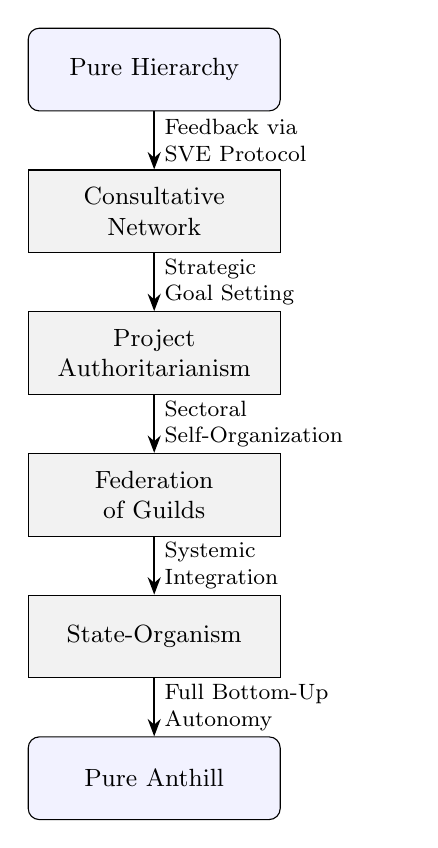
\begin{tikzpicture}[node distance=1.8cm, auto]
\node (hierarchy) [startstop] {Pure Hierarchy};
\node (consultative) [process, below of=hierarchy] {Consultative\\Network};
\node (project) [process, below of=consultative] {Project\\Authoritarianism};
\node (guilds) [process, below of=project] {Federation\\of Guilds};
\node (organism) [process, below of=guilds] {State-Organism};
\node (anthill) [startstop, below of=organism] {Pure Anthill};

% Arrows with labels
\draw [arrow] (hierarchy) -- node[right, font=\footnotesize, text width=3cm, align=left] {Feedback via\\SVE Protocol} (consultative);
\draw [arrow] (consultative) -- node[right, font=\footnotesize, text width=3cm, align=left] {Strategic\\Goal Setting} (project);
\draw [arrow] (project) -- node[right, font=\footnotesize, text width=3cm, align=left] {Sectoral\\Self-Organization} (guilds);
\draw [arrow] (guilds) -- node[right, font=\footnotesize, text width=3cm, align=left] {Systemic\\Integration} (organism);
\draw [arrow] (organism) -- node[right, font=\footnotesize, text width=3cm, align=left] {Full Bottom-Up\\Autonomy} (anthill);
\end{tikzpicture}
\caption{Spectrum of Hybrid Governance Models, from Hierarchy to Anthill, with increasing self-organization. Each transition represents deeper integration of the Epistemological Boxing Protocol \citep{Kovnatsky2025Boxing}.}
\label{fig:hybrid_spectrum}
\end{figure}

% --- Enhanced radar chart with hybrid overlay ---
\begin{figure}[h!]
\centering
\begin{tikzpicture}
\begin{polaraxis}[
  width=0.7\textwidth,
  height=0.7\textwidth,
  title={Hybrid Model: Combining Strengths of Both Systems},
  theta zero=90,
  theta direction=clockwise,
  ymin=0, ymax=100,
  xtick={0,72,144,216,288},
  xticklabels={Stability, Adaptability, Engagement, Speed, Resilience},
  ytick={0,20,40,60,80,100},
  grid=both,
  major grid style={draw=gray!40},
  minor grid style={draw=gray!20},
  ticklabel style={font=\small},
  title style={font=\normalsize\bfseries, yshift=0.3cm},
  legend cell align=left,
  legend style={draw=none, font=\small, at={(1.25,0.5)}, anchor=west},
  every axis plot/.append style={line width=1.4pt, mark=*, mark size=2.5pt},
  set layers=standard
]

% Hybrid model (best of both) - in background
\addplot+[
  on layer=axis background,
  draw={RGB}{230,159,0},
  fill={RGB}{230,159,0}, 
  fill opacity=0.15,
  line width=1.8pt,
  mark size=2pt
] coordinates {
  (0,90) (72,90) (144,80) (216,85) (288,95) (360,90)
};
\addlegendentry{Hybrid (optimal)}

% Hierarchy
\addplot+[
  draw={RGB}{0,114,178}, 
  fill={RGB}{0,114,178}, 
  fill opacity=0.18
] coordinates {
  (0,90) (72,30) (144,20) (216,85) (288,15) (360,90)
};
\addlegendentry{Hierarchy}

% Anthill
\addplot+[
  draw={RGB}{213,94,0}, 
  fill={RGB}{213,94,0}, 
  fill opacity=0.18
] coordinates {
  (0,25) (72,90) (144,80) (216,35) (288,95) (360,25)
};
\addlegendentry{Anthill}

\end{polaraxis}
\end{tikzpicture}
\caption{Hybrid governance models achieve superior performance by combining the complementary strengths of hierarchical stability and anthill adaptability, as demonstrated by the optimal envelope (yellow) encompassing the best attributes of both pure systems.}
\label{fig:hybrid_comparison}
\end{figure}

% --- SECTION 4: INSURANCE MECHANISMS ---
\section{Systemic Insurance Mechanisms for Antifragility}
To ensure resilience, hybrid models incorporate the following mechanisms:

\begin{description}[style=nextline, leftmargin=0pt, labelindent=0pt]
    \item[\textbf{Skin in the Game}] Decision-makers face financial liability for errors, ensuring accountability and alignment of incentives \citep{Taleb2018,HybridModelsMemo}.
    
    \item[\textbf{Right to Neat Chaos}] Small-scale experiments foster innovation and learning from controlled failures, enabling the system to gain from disorder \citep[lines 2315--2316]{HybridModelsMemo}.
    
    \item[\textbf{Institute of ``Holy Fools'' (Yurodivy)}] Protected critics speak truth to power without fear of retaliation, maintaining epistemic diversity \citep[lines 2317]{HybridModelsMemo}.
    
    \item[\textbf{Parallel Structures}] Redundant institutions prevent truth monopolies and provide alternative pathways for decision-making \citep[lines 2318]{HybridModelsMemo}.
\end{description}

% --- SECTION 5: DISCUSSION ---
\section{Discussion: Missing Links and Implementation Pathway}
Successful implementation requires addressing three critical challenges:

\subsection{The Translator Problem}
Bridging the Hierarchy's directives and the Anthill's values requires sophisticated translation mechanisms—either AI systems or trained human intermediaries capable of bidirectional communication \citep[lines 2320--2322]{HybridModelsMemo}.

\subsection{The New Human Problem}
Educational reform is essential to cultivate citizens capable of engaging with the Boxing Protocol, emphasizing critical thinking, epistemic humility, and collaborative truth-seeking \citep[lines 2323--2326]{HybridModelsMemo}.

\subsection{Guardians of the Method Problem}
An independent ``Supreme Court of Meaning'' must oversee SVE integrity, preventing capture or corruption of the truth-seeking process itself \citep[lines 2327--2331]{HybridModelsMemo}.

\subsection{Implementation Strategy}
Begin with the Consultative Network (Model 1) as a minimum viable approach, iteratively advancing to more complex models as institutions mature and trust develops \citep[lines 2335--2336]{HybridModelsMemo}. This evolutionary pathway allows for learning and adaptation at each stage.

% --- SECTION 6: CONCLUSION ---
\section{Conclusion}
Hybrid governance models, enabled by the SVE framework, offer a viable pathway to antifragile, truth-oriented states. The \textit{Socratic tail}—characterized by epistemic humility and iterative learning—underpins their adaptability and resilience. These models are not static ideals but dynamic vectors for evolution, ensuring societal survival through institutionalized truth-seeking \citep[lines 2337--2338]{HybridModelsMemo}. By synthesizing hierarchical efficiency with distributed innovation, they transcend the false dichotomy that has constrained governance theory for centuries.

% --- BIBLIOGRAPHY ---
\bibliographystyle{plainnat}
\bibliography{\jobname}

% --- APPENDIX ---
\clearpage
\appendix

% --- VISUALIZATION APPENDIX ---
\section{Visualization of Hybrid Governance Models}
\label{app:visualization}

This appendix presents the key visualizations referenced in the main text. Figure~\ref{fig:hybrid_spectrum} illustrates the evolutionary pathway from pure Hierarchy to pure Anthill through four intermediate hybrid models. Figure~\ref{fig:hybrid_comparison} demonstrates how hybrid approaches achieve superior performance across all governance dimensions by combining complementary strengths.


% --- Appendix A: The Defiant Manifesto: The Scientific Protocol vFinal ---
\clearpage % Start on a new page

% Define colors if not already defined
\providecolor{headercolor}{RGB}{0, 51, 102}
\providecolor{accentcolor}{RGB}{0, 102, 204}


\section*{Appendix A. The Defiant Manifesto: The Scientific Protocol}
\addcontentsline{toc}{section}{Appendix A. The Defiant Manifesto: The Scientific Protocol}
\label{app:manifesto}

\vspace{1em}

\noindent\fcolorbox{accentcolor}{gray!5}{%
\begin{minipage}{\dimexpr\textwidth-2\fboxsep-2\fboxrule}
\textit{This appendix translates the moral courage of the original political manifesto into scientific clarity. Where politics defends through rhetoric, Systemic Verification Engineering (SVE) defends through reason. It embodies the \textbf{Socratic principle} by embracing critique as a catalyst for its own evolution. The text below specifies the philosophical antibodies of SVE—a self-healing discipline designed to thrive on challenge.}
\end{minipage}}

\vspace{1.5em}

\noindent\textbf{\textcolor{headercolor}{Core Premise.}} Their weapon is the appeal to captured authority. Our weapons are open methodology, logical rigor, radical transparency, and unwavering faith in the power of Truth. This document, like the SVE Protocol itself, is a living artifact; it will be publicly updated as new intellectual challenges emerge, turning every attack into evidence of its necessity and a catalyst for its reinforcement.

\vspace{1em}

% Scientific Lineage
\subsection*{\textcolor{headercolor}{Scientific Lineage}}
SVE stands in a lineage of transformative disciplines initially dismissed by the establishment: Darwinism (``pseudoscience''), Cybernetics (``ideology''), early Computer Science (``mere theory''). Each reshaped the paradigm it challenged. SVE follows this path: not a rejection of science, but its rehabilitation through verifiability, self-audit, and institutional design grounded in epistemic humility.

\vspace{1em}

% Attack 1
\subsection*{\textcolor{accentcolor}{Attack 1: ``This is Pseudoscience''}}

\paragraph{\textbf{Claim.}} SVE is non-rigorous; the ``Theorem on Disaster Prevention'' is a socio-probabilistic metaphor, not real mathematics; TRIZ is misapplied.

\paragraph{\textbf{Our Shield (Explanatory Power).}} We concede the Theorem is not pure mathematics; it is a \textbf{foundational axiom for an applied discipline}. Its validity stems from its predictive and explanatory power: modeling democracy as ``guessing the weight of an ox behind a closed door with expert labels'' accurately diagnoses real-world systemic failures (e.g., the Iraq War justification, the 2008 financial crisis, contradictory pandemic policies). SVE earns epistemic status by \textit{outperforming} existing institutional explanations in fidelity to observable outcomes.

\paragraph{\textbf{Our Counter (Public Intellectual Challenge).}} We invite critics to a live, recorded, long-form \textbf{epistemological boxing match}. They may deconstruct our methods under the SVE protocol itself; we will, in turn, apply the same protocol to audit the systemic failures their paradigms normalize. Let the public judge which approach better serves society: descriptive justifications from within a failing system, or an engineering blueprint designed to fix it.

\vspace{1em}

% Attack 2
\subsection*{\textcolor{accentcolor}{Attack 2: ``This is Ideology Disguised as Science''}}

\paragraph{\textbf{Claim.}} Christian ethics and concepts like ``multiplying love'' reveal inherent bias; the project is dogma masquerading as science.

\paragraph{\textbf{Our Shield (Architectural Separation of Fact and Value).}} SVE's three-stage architecture deliberately separates verifiable facts (\textit{``Caesar's realm''}) from value judgments (\textit{``God's realm''}). The protocol does not dictate morality; it secures a verified factual substrate upon which citizens can conduct informed deliberation. A scalpel in a Christian surgeon's hand remains a scalpel; function is defined by design and intent, not the wielder's faith.

\paragraph{\textbf{Our Counter (Demand for First Principles).}} We challenge critics to explicitly state the moral axioms underlying the status quo, which often tolerates dehumanizing logic (e.g., ``human resources,'' ``collateral damage''). Science devoid of declared ethics is not neutral; it is merely a tool available for hire by the highest bidder. We state our principles—rooted in the pursuit of truth and love—openly, and challenge others to do the same.

\vspace{1em}

% Attack 3
\subsection*{\textcolor{accentcolor}{Attack 3: ``This is Dangerous Science'' (The ``Ministry of Truth'' Gambit)}}

\paragraph{\textbf{Claim.}} A protocol capable of verifying truth could be weaponized by future tyrants to enforce a single narrative.

\paragraph{\textbf{Our Shield (Limited by Design \& Decentralized Trust).}} SVE is architected for \textbf{self-dissolution and decentralization}. The implementing institution (e.g., PFP party, SVE Foundation) is designed to create the tools, transfer copyright and control to a decentralized structure (the SVE DAO governed by a global community), and then disappear. It is the antithesis of a self-perpetuating ministry; it is a self-terminating catalyst for distributed verification.

\paragraph{\textbf{Our Counter (The True Danger is the Unverified Lie).}} The present and clear danger is not verified truth, but systemic, unchallengeable falsehood that paralyzes effective problem-solving and enables catastrophes. A democracy poisoned by lies is already a tyranny in disguise—a ``Ministry of Lies'' captured by hidden interests. SVE builds a shield for citizens against the tyranny that \textit{already exists}: the tyranny of the unaccountable lie.

\vspace{1em}

% Attack 4
\subsection*{\textcolor{accentcolor}{Attack 4: ``This is Politicized Science''}}

\paragraph{\textbf{Claim.}} Science is inherently contested and politicized (e.g., COVID-19, climate change); no objective protocol can arbitrate truth.

\paragraph{\textbf{Our Shield (Radical Honesty about Systemic Failure).}} We agree unequivocally: establishment science \textit{has been} deeply politicized and captured. This capture is not an argument against independent verification—it is the \textbf{primary justification} for it.

\paragraph{\textbf{Our Counter (The Protocol is the Cure, Not the Disease).}} SVE does not add another biased expert opinion to the fray. It installs a \textbf{meta-structure} that audits the experts themselves, separates factual claims from political spin, and publishes transparent, reproducible audit trails. We are not entering the political fight \textit{as} scientists fighting for a particular outcome; we are applying engineering principles to repair the fundamentally broken \textit{process} by which science informs public life.

\vspace{1em}

% Attack 5
\subsection*{\textcolor{accentcolor}{Attack 5: ``This is Too Complex for the People''}}

\paragraph{\textbf{Claim.}} Theorems, protocols, DAOs—this is too complex for ordinary citizens; inherently elitist.

\paragraph{\textbf{Our Shield (Distinguishing Complexity from Obfuscation).}} Modern life is complex (e.g., car engines, smartphones), but good design provides simple interfaces (steering wheels, touchscreens). The status quo often weaponizes complexity as \textbf{obfuscation} to prevent accountability. SVE distinguishes necessary internal complexity (the engineering under the hood) from deliberate external opacity.

\paragraph{\textbf{Our Counter (The Complexity Translator).}} The Socratic AI assistants and the three-stage architecture are explicitly designed to act as \textbf{complexity translators}. They distill intricate realities into: (1) Verifiable factual building blocks, (2) A clear spectrum of expert interpretations and value judgments, and (3) An understandable basis for civic choice. We do not demand citizens become engineers; we empower them with a reliable steering wheel for navigating complexity.

\vspace{1em}

% Attack 6
\subsection*{\textcolor{accentcolor}{Attack 6: ``This Will Stifle Innovation''}}

\paragraph{\textbf{Claim.}} Rigorous verification requirements will slow down scientific progress and punish creative, unconventional ideas.

\paragraph{\textbf{Our Shield (Correction, Not Punishment; Contextual Rigor).}} The protocol's 44-day grace period and emphasis on intellectual honesty foster a culture of learning from error, not fear of it. Bold hypotheses are encouraged; fabricated data is not. Furthermore, the level of required rigor is contextual: exploratory research faces a different standard than clinical trial data determining public health policy.

\paragraph{\textbf{Our Counter (Innovation Requires a Solid Foundation).}} True scientific progress is slowed far more by building upon fraudulent or irreproducible findings than by careful verification. Chasing phantom results based on bad data wastes decades and billions. SVE accelerates meaningful progress by ensuring each step rests on solid ground. Trust is the lubricant of innovation.

\vspace{1em}

% Attack 7
\subsection*{\textcolor{accentcolor}{Attack 7: ``This is Arrogant Science''}}

\paragraph{\textbf{Claim.}} Claiming to approximate objective truth is intellectual hubris, especially in light of postmodern critiques showing the social construction of knowledge.

\paragraph{\textbf{Our Shield (Epistemic Humility Architected In).}} SVE explicitly rejects claims of absolute truth. It produces \textit{Iterative Facts}—version-controlled, provisional, falsifiable conclusions, each carrying a fully documented, publicly auditable chain of reasoning and acknowledged limitations. The protocol's strength lies precisely in its \textbf{institutionalized admission of fallibility}. It aims for the most reliable approximation of truth currently possible, knowing it will be superseded.

\paragraph{\textbf{Our Counter (What Constitutes True Arrogance?).}} True arrogance lies in the current system: anonymous reviewers wielding unaccountable power, captured agencies declaring safety without independent scrutiny, media monopolies acting as arbiters of truth without transparent methodology. SVE proposes radical transparency where opacity now reigns, falsifiability against dogma, and public accountability replacing impunity. Is it arrogant to demand that claims affecting millions of lives be verifiable?

\vspace{1.5em}

% Closing Principle
\subsection*{\textcolor{headercolor}{Closing Principle: Reflexive Truth and Service}}

Every valid system must contain a mechanism to question and correct itself. SVE institutionalizes this reflex: the permanent, transparent audit of power, of science, and critically, \textit{of its own conclusions}. In this paradox lies its incorruptibility: by structurally embracing its own fallibility, it becomes resistant to dogma and capture.

The Protocol is not a fortress built to defend a final truth; it is a mirror designed to reflect reality more clearly, iteration by iteration. It does not seek to win the argument, but to keep the argument honest, tethered to facts and logic. Its ultimate aim is not intellectual victory, but service—service to the truth, and through truth, service to love and the flourishing of all.

\vspace{2em}

% Quotes section with better spacing
\begin{center}
\begin{minipage}{0.9\textwidth}
\hrule height 0.5pt
\vspace{1em}

\noindent\textit{``Judge not, that you be not judged.''} --- Matthew 7:1

\vspace{0.6em}
\noindent\textit{``I know that I know nothing.''} --- Socrates

\vspace{0.6em}
\noindent\textit{``The first principle is that you must not fool yourself—and you are the easiest person to fool.''} --- Richard Feynman

\vspace{0.6em}
\noindent\textit{``In a time of deceit, telling the truth is a revolutionary act.''} --- Often attributed to George Orwell

\vspace{1em}
\hrule height 0.5pt
\vspace{1em}

{\fontencoding{T2A}\selectfont
\noindent\textit{«Учітеся, брати мої,\\
Думайте, читайте,\\
І чужому научайтесь,\\
Й свого не цурайтесь...»}\\
--- Т. Шевченко («І мертвим, і живим, і ненарожденним...», 1845)

\vspace{0.8em}
\noindent\textit{«Скажи мне, американец, в чём сила? Разве в деньгах? [...] А я вот думаю, что сила — в правде. У кого правда — тот и сильней.»}\\
--- Д. Багров / Сергей Бодров-мл. (\href{https://youtu.be/fz6lGsgEGZ8}{«Брат 2»})
}

\vspace{1em}
\hrule height 0.5pt
\vspace{1em}

\noindent\textit{Father, guide us, Your children, on the path of truth; teach us to love—ourselves and our neighbors.}

\vspace{0.8em}
\noindent\textit{«I am the way, and the truth, and the life.»} --- John 14:6

\vspace{0.4em}
\noindent\textit{«You shall love your neighbor as yourself.»} --- Matthew 22:39

\vspace{1em}
\noindent\textit{Soli Deo gloria.} (Glory to God alone.)

\vspace{0.5em}
\hrule height 0.5pt
\end{minipage}
\end{center}

% --- END Appendix A ---

\end{document}